\documentclass[spanish,12pt,letterpaper]{article}
\usepackage[T1]{fontenc}
\usepackage[left=1cm, right=1cm, top=2cm, bottom=2cm]{geometry}
\usepackage{graphicx}
\usepackage{tikz}
\usetikzlibrary{arrows.meta, shapes.geometric, positioning, babel}
\usepackage{pgfplots}
\pgfplotsset{compat=1.18}
\usepgfplotslibrary{polar, colorbrewer, statistics}
\pgfplotsset{
	compat=1.18,
	width=10cm,
	height=6cm
}
\usepgfplotslibrary{groupplots}
\usepgfplotslibrary{fillbetween}
\usepackage{mathtools}
\usepackage{amssymb}
\usepackage{amsthm}
\usepackage{thmtools}
\usepackage{xcolor}
\usepackage{nameref}
\usepackage{babel}
%\usepackage{Babel}
%\usepackage{hyperref}
\title{Aplicacione De Comandos Entornos Librerías-PGFPlots}
\author{Toribio}
\begin{document}
	\maketitle
	
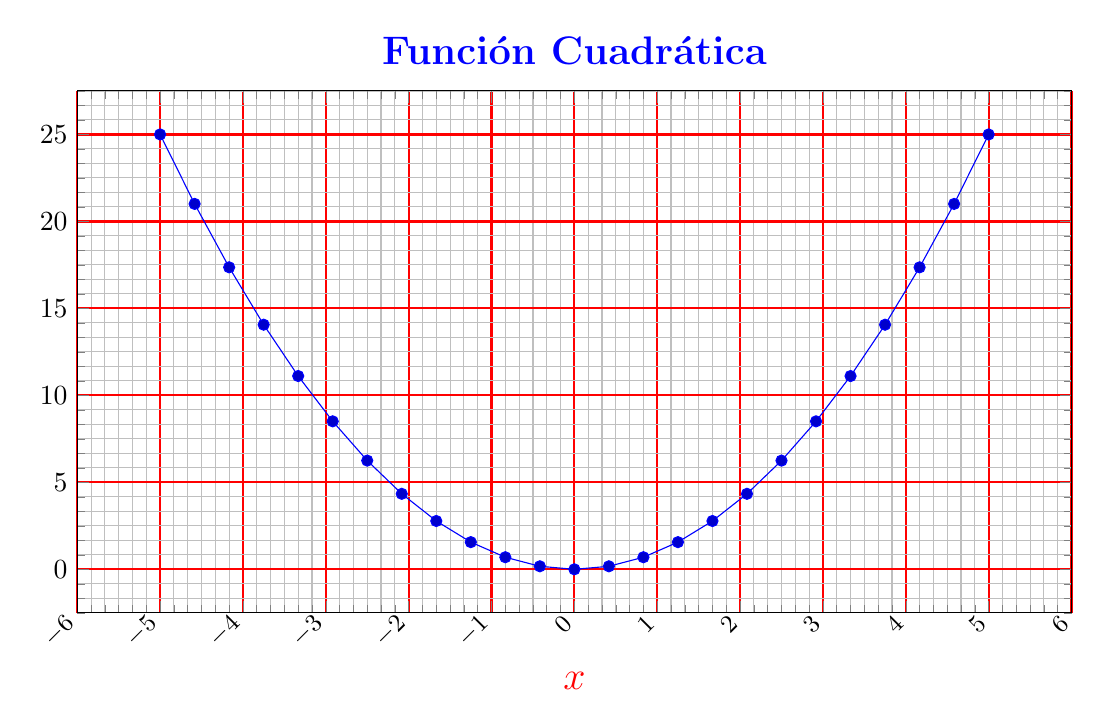
\begin{tikzpicture}
	\begin{axis}[scale=1.5, grid=both,
		major grid style={thick, red}, xlabel=$x$,
		xlabel style={font=\Large, color=red}, title=Función Cuadrática, title style={font=\bfseries\Large, color=blue}, minor tick num=5, xticklabel style={rotate=45, anchor=east, font=\small}]
		\addplot {x^2};
	\end{axis}
\end{tikzpicture} \\[3mm]

\begin{tikzpicture}
	\begin{axis}[scale=1.5]
		\addplot {sin(deg(x))};
	\end{axis}
\end{tikzpicture} \\[3mm]

\begin{tikzpicture}
	\begin{axis}[scale=1.5]
		\addplot {x};
	\end{axis}
\end{tikzpicture} \\[3mm]

\begin{tikzpicture}
	\begin{axis}[xmin=0, xmax=10, ymin=-3, ymax=3, scale=1.5]
		\addplot {sin(deg(x))};
	\end{axis}
\end{tikzpicture} \\[3mm]

\begin{tikzpicture}
	\begin{axis}[scale=1.5]
		\addplot[domain=-2:2] {x^3};
	\end{axis}
\end{tikzpicture} \\[3mm]

\begin{tikzpicture}
	\begin{axis}[scale=1.5]
	\addplot[restrict y to domain=-10:10] {1/x};
	\end{axis}
\end{tikzpicture} \\[3mm]

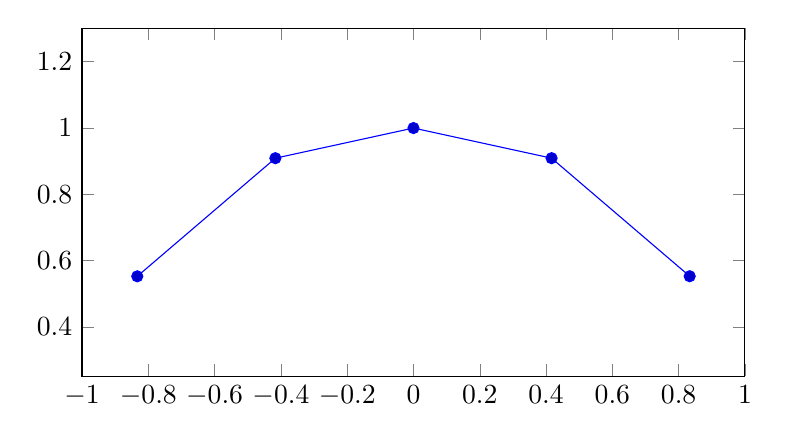
\begin{tikzpicture}
	\begin{axis}[axis equal]
		\addplot {sqrt(1-x^2)};
	\end{axis}
\end{tikzpicture} \\[3mm]

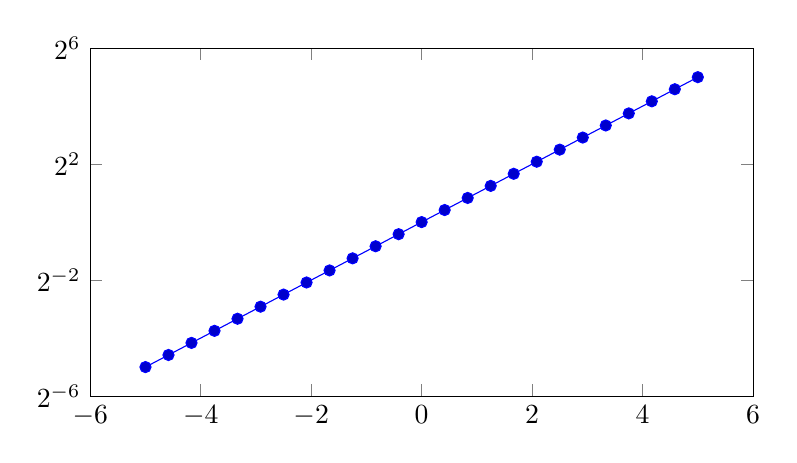
\begin{tikzpicture}
	\begin{axis}[ymode=log, log basis y=2]
		\addplot {2^x};
	\end{axis}
\end{tikzpicture} \\[3mm]

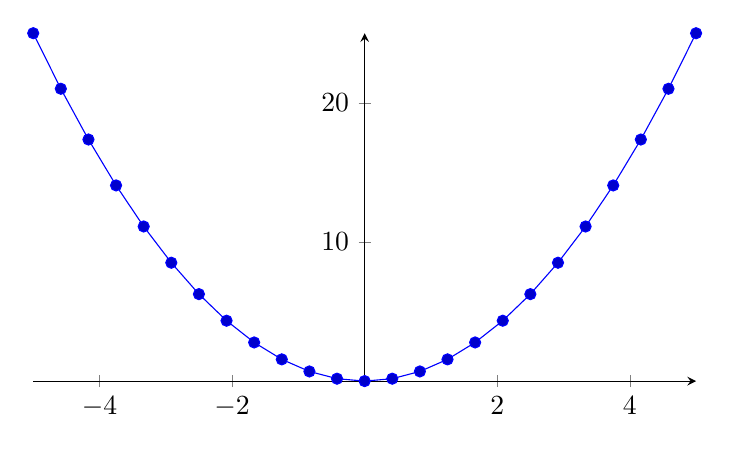
\begin{tikzpicture}
	\begin{axis}[axis x line=middle, axis y line=center]
		\addplot {x^2};
	\end{axis}
\end{tikzpicture} \\[3mm]

\begin{tikzpicture}
	\begin{axis}[axis lines=center]
		\addplot[smooth] {sin(deg(x))};
	\end{axis}
\end{tikzpicture} \\[3mm]

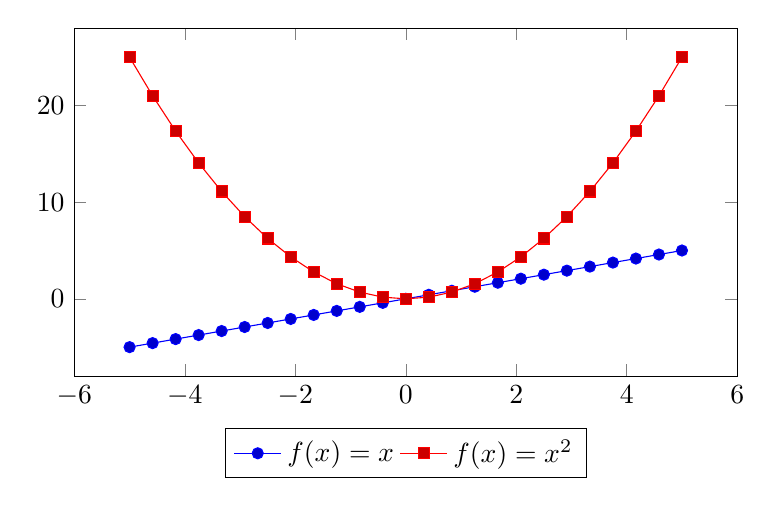
\begin{tikzpicture}
	\begin{axis}[legend style={at={(0.5,-0.15)}, anchor=north,
			legend columns=2}]
		\addplot {x}; \addlegendentry{$f(x)=x$} 
		\addplot {x^2}; \addlegendentry{$f(x)=x^2$}
	\end{axis}
\end{tikzpicture} \\[3mm]

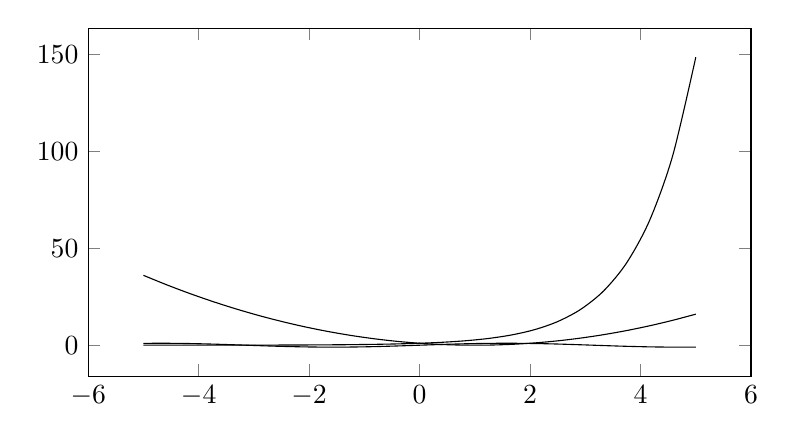
\begin{tikzpicture}
	\begin{axis}
		\addplot[smooth] {x^2 - 2*x + 1};
		\addplot[smooth] {sin(deg(x))};
		\addplot[smooth] {exp(x)};
	\end{axis}
\end{tikzpicture} \\[3mm]

\begin{tikzpicture}
	\begin{axis}
		\addplot3[samples=200] {x^2 + y^2};
	\end{axis}
\end{tikzpicture} \\[3mm]

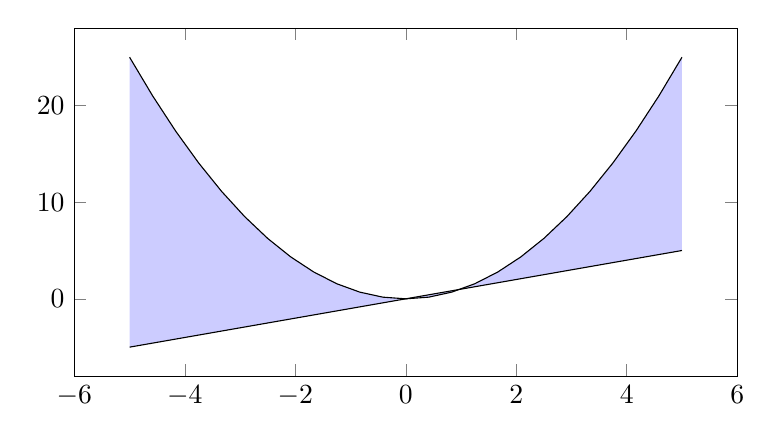
\begin{tikzpicture}
	\begin{axis}
		\addplot[name path=A] {x^2};
		\addplot[name path=B] {x};
		\addplot[fill=blue!20] fill between[of=A and B];
	\end{axis}
\end{tikzpicture} \\[3mm]

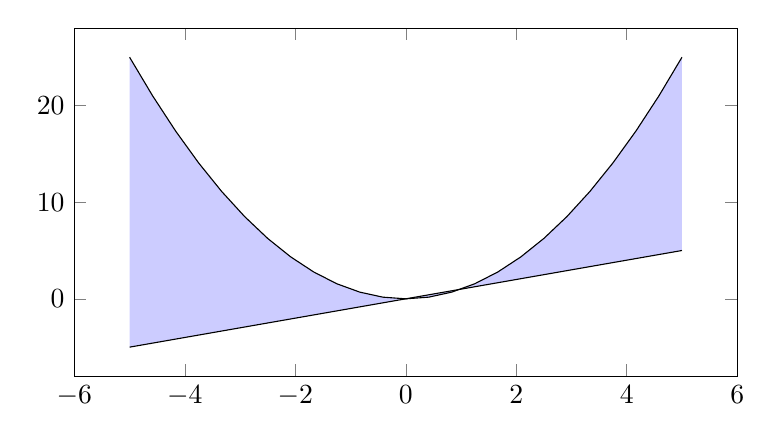
\begin{tikzpicture}
	\begin{axis}
		\addplot[name path=A] {x^2};
		\addplot[name path=B] {x};
		\addplot[fill=blue!20] fill between[of=A and B];
	\end{axis}
\end{tikzpicture} \\[3mm]

\begin{tikzpicture}
	\begin{groupplot}[group style={group size=2 by 2}]
		\nextgroupplot
		\addplot[smooth] {x};
		\nextgroupplot
		\addplot[smooth] {x^2};
	\end{groupplot}
\end{tikzpicture}
	
\end{document}